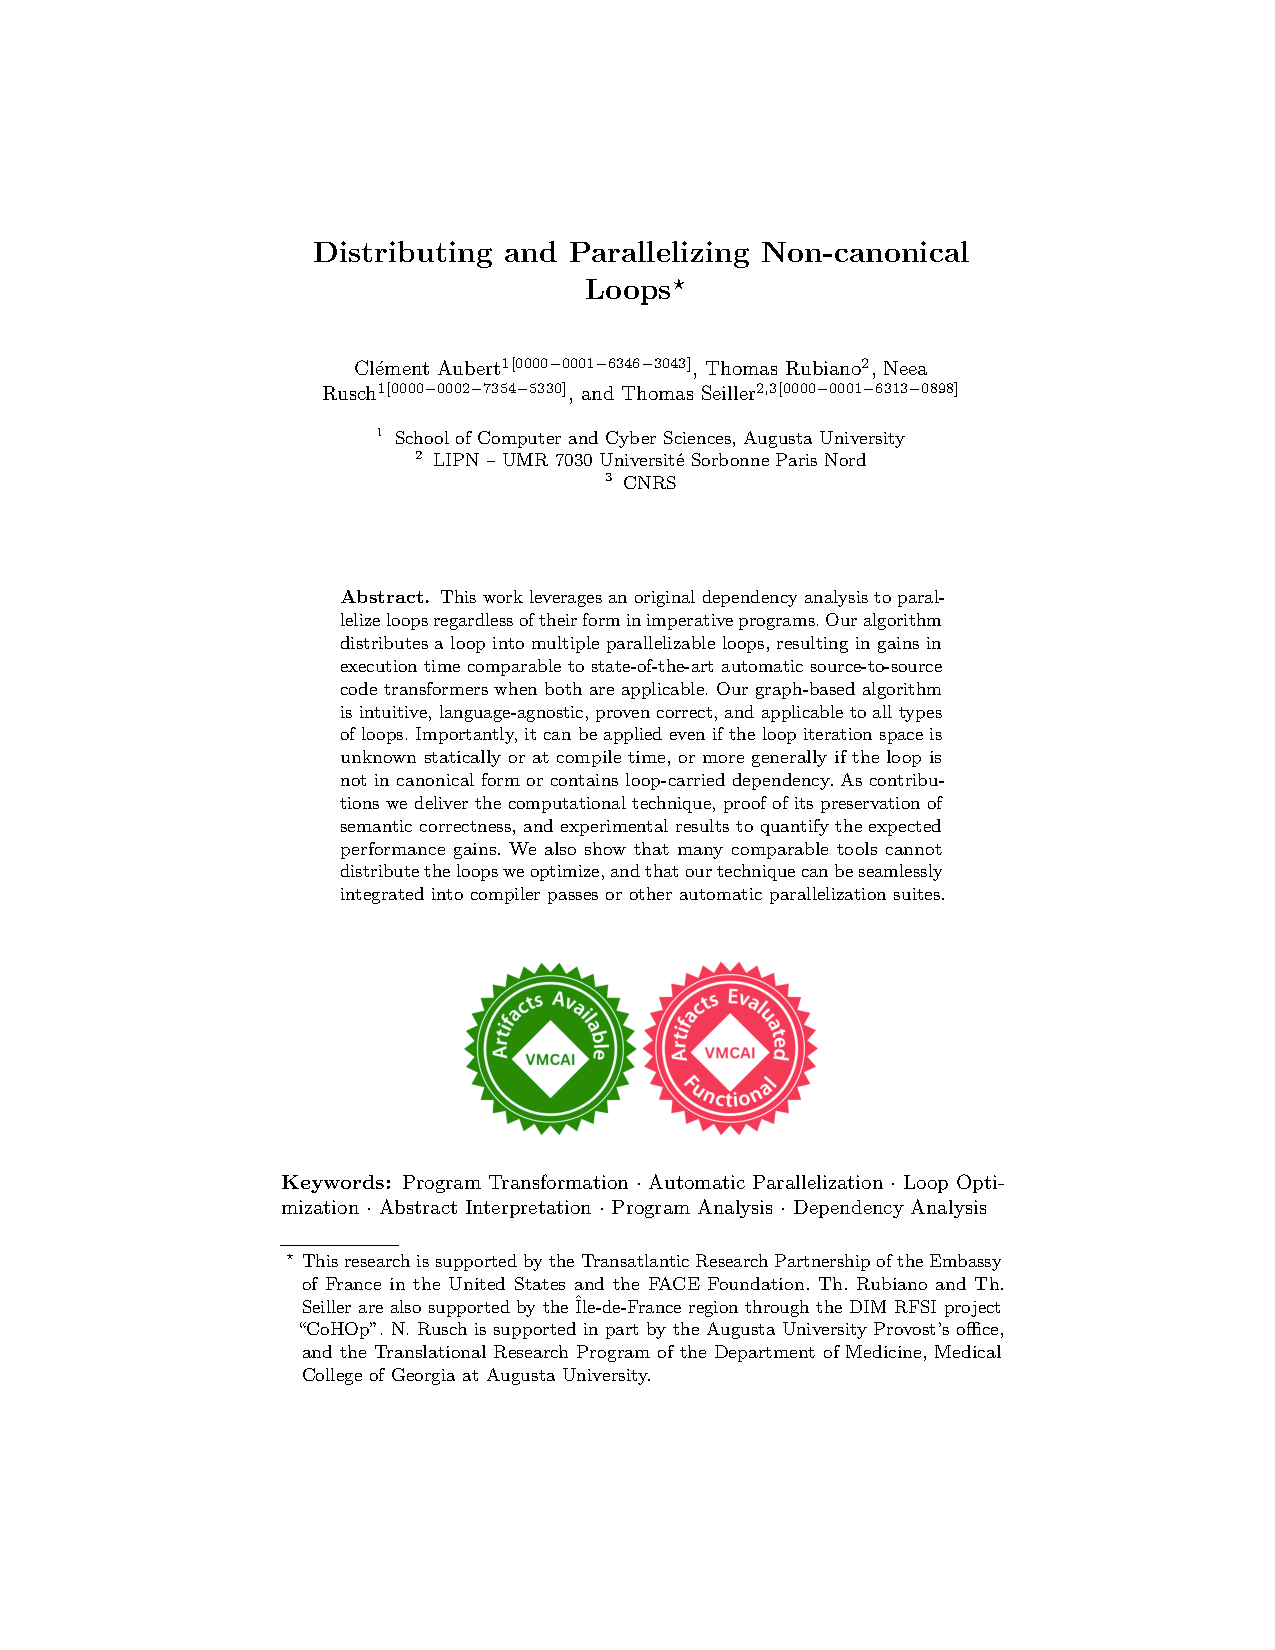
\includepdf[pages={1-},
    addtotoc={
        2,subsection,2,{Original Approaches to Automatic Parallelization},sec:vmcai-intro,
        4,subsection,2,{Background: Language and Dependency Analysis},sec:vmcai-background,
        11,subsection,2,{Loop Fission Algorithm},sec:fission-algo,
        14,subsection,2,{Limitations of Existing Alternative Approaches},sec:vmcai-limitations,
        16,subsection,2,{Evaluation},sec:vmcai-eval,
        21,subsection,2,{Conclusion},sec:vmcai-conc},
    addtolist={
        5,figure,{Simple imperative while language},fig-grammar,
        6,table,{Definition of Out, In and Occ for commands},table:def-out-in-occ,
        8,figure,{Statement examples, sets, and representations of their dependencies},fig:dependences,
        9,figure,{Data-Flow Graph of composition},fig:composition,
        12,algorithm,{A loop fission algorithm for parallelizing loops},alg:loop-fission,
        13,figure,{Distributing a more complex while loop},fig:example-complex,
        16,table,{Parallelization tools feature support comparison},tab:comparison,
        17,figure,{Code transformation example},fig:code-example,
        19,figure,{Speedup of selected benchmarks},fig:while,
        20,table,{Speedup comparison between parallel benchmarks},tab:speedup,
        20,table,{Descriptions of evaluated parallel benchmarks},tab:benchmarks},
    pagecommand={\thispagestyle{empty}%
    \addtoindexm{C++}{15}
    \addtoindexm{CPU}{18}
    \addtoindexm{Cetus}{15,16}
    \addtoindexm{Clava}{15,16,19}
    \addtoindexm{C}{15,16,18}
    \addtoindexm{GCC compiler}{14,18}
    \addtoindexm{Intel's C++ compiler}{15,16}
    \addtoindexm{LLVM compiler}{14}
    \addtoindexm{MiBench}{17,20}
    \addtoindexm{NAS Parallel Benchmarks}{17,20}
    \addtoindexm{OpenMP directives!nowait}{17}
    \addtoindexm{OpenMP directives!parallel}{5,15,16,17}
    \addtoindexm{OpenMP directives!pragma omp}{17}
    \addtoindexm{OpenMP directives!private}{17}
    \addtoindexm{OpenMP directives!single}{17,18}
    \addtoindexm{OpenMP}{2,3,4,14,15,16,18,19,20}
    \addtoindexm{Par4All}{15,16}
    \addtoindexm{Pluto}{15,16}
    \addtoindexm{Polybench/C}{16,17,18}
    \addtoindexm{ROSE}{14,15,16,17,18,9,20}
    \addtoindexm{TRACO}{15,16}
    \addtoindexm{automatic parallelization}{3,4,15,16,19,20}
    \addtoindexm{bi-partite graph}{7}
    \addtoindexm{canonical loop}{2,4,15,16,17}
    \addtoindexm{compiler!GCC}{14,18}
    \addtoindexm{compiler!LLVM}{14}
    \addtoindexm{compiler!ROSE}{14,15,16,17,18,19,20}
    \addtoindexm{compiler!icc}{15,16}
    \addtoindexm{condensation graph}{11,12,13}
    \addtoindexm{data-flow graph}{6,7}
    \addtoindexm{dependence graph}{11,14,15}
    \addtoindexm{dependence analysis}{2,4,6,14,21}
    \addtoindexm{graph covering}{11,12,13,14}
    \addtoindexm{intermediate representation}{3}
    \addtoindexm{iteration space}{1,2,3,4,6,13,14,18,19}
    \addtoindexm{loop transformation!distribution}{2}
    \addtoindexm{loop transformation!fission}{2,3,4,6,11,12,14,15,16,17,18,19,20}
    \addtoindexm{loop transformation!fusion}{21}
    \addtoindexm{loop transformation!tiling}{4}
    \addtoindexm{loop transformation!unrolling}{3,21}
    \addtoindexm{loop-carried dependency}{15}
    \addtoindexm{loop-level parallelism}{2}
    \addtoindexm{nested loop}{11}
    \addtoindexm{non-canonical loop}{2,21}
    \addtoindexm{parallel programming}{2,3,17}
    \addtoindexm{parallelization directive}{3,4,5,16,18,19,20}
    \addtoindexm{parallelization potential}{3}
    \addtoindexm{parallelizing compilation}{3,15,16,17,19}
    \addtoindexm{polyhedral optimization}{4}
    \addtoindexm{programming language!C++}{15}
    \addtoindexm{programming language!C}{15}
    \addtoindexm{saturated covering}{12,13}
    \addtoindexm{source-to-source compilation}{1,3,15}
    \addtoindexm{state explosion}{3}
    \addtoindexm{structured block}{15}
    \addtosymbolsm{corro}{9}
    \addtosymbolsm{corr}{8,9,10}
    \addtosymbolsm{dfg}{7,8,10,11}
    \addtosymbolsm{et}{9}
    \addtosymbolsm{graphw}{11,12}
    \addtosymbolsm{graph}{12}
    \addtosymbolsm{infty2}{7,8,9,10,11}
    \addtosymbolsm{looppw}{12,13,14}
    \addtosymbolsm{loopw}{10,11,12,13,14}
    \addtosymbolsm{mdfg}{7,8,9,10,11,13}
    \addtosymbolsm{occ}{6,7,9,10}
    \addtosymbolsm{one}{7,8,9,10}
    \addtosymbolsm{vin}{6,7,8,11}
    \addtosymbolsm{vout}{6,7,8,9,10,11}
    \addtosymbolsm{zero2}{7,8,9,10}
    }]{pdf/pubs_vmcai.2023.pdf}